\documentclass[a4paper]{article}
\usepackage{Sweave}
\usepackage[margin=2cm]{geometry}
\usepackage[round]{natbib}
\usepackage{url}
\usepackage{hyperref}
\usepackage{listings}

\let\code=\texttt
\newcommand{\acronym}[1]{\textsc{#1}}
\newcommand{\class}[1]{\mbox{\textsf{#1}}}
\newcommand{\pkg}[1]{{\normalfont\fontseries{b}\selectfont #1}}
\newcommand{\proglang}[1]{\textsf{#1}}
\newcommand{\fkt}[1]{\code{#1}}
\newcommand{\todo}[1]{\begin{center}\code{<TODO: #1>}\end{center}}    
\newcommand{\field}[1]{\code{\$#1}} 
 
\sloppy
%% \VignetteIndexEntry{Introduction to the tm.plugin.webmining Package}
 



\begin{document}

 
\title{Introduction to \pkg{tm.plugin.webmining}}
\author{Mario Annau\\
		\texttt{mario.annau@gmail.com}}

\maketitle
   
\abstract{
This vignette gives an introduction to \pkg{tm.plugin.webmining}, 
an add-on package to \pkg{tm} which facilitates the retrieval of textual 
data from the web. The main focus of \pkg{tm.plugin.webmining} is the retrieval
of web content from structured news feeds in the \proglang{XML} (\proglang{RSS}, \proglang{ATOM}) and
\proglang{JSON} format. Furthermore, the direct retrieval through  \proglang{HTML}
documents is implemented. Numerous data sources are supported, including Google--,Yahoo!-- and 
Bing News, Reuters, New York Times, Twitter, etc. In addition to simple feed content retrieval,
also the complete source articles can be downloaded and extracted through \pkg{RCurl} and
\pkg{boilerpipeR}.
}

\tableofcontents
\newpage  
  
\section{Introduction}
\pkg{tm.plugin.webmining} facilitates the retrieval of web content through news feeds. Feeds typically provide
up--to--date information from content providers in a standardized format for easy parsing. The main advantage
of using content from news feeds is that it already provides meta data like the Date--/Timestamp, Author and other
useful information. Since all new information is only published through the news feed, it is also easier to track
changes of a



 in stan \proglang{RSS}, \proglang{}




\section{Package Overview}
\begin{figure}[tbp]
\centering
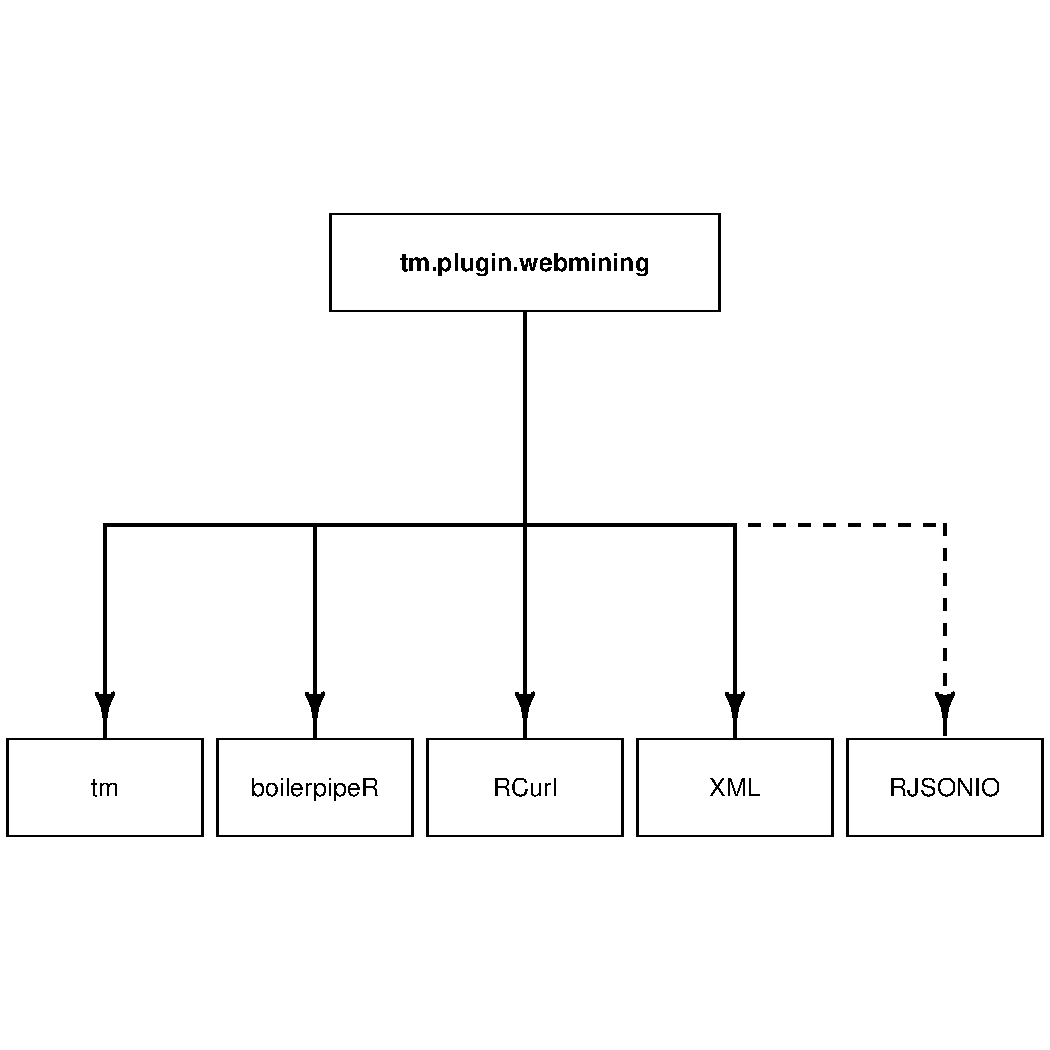
\includegraphics[width = 8cm]{figures/dependenceplot}
\caption{	Illustration of the \pkg{tm.plugin.webmining} package dependencies. Solid lines 
			indicate dependencies, dashed lines imports (as indicated by the package DESCRIPTION file).
			Figure created using \pkg{diagram}.
}
\label{fig:schema_tm.plugin.webmining}
\end{figure}

To enable a wide range of web data retrieval use cases \pkg{tm.plugin.webmining} uses functions
from numerous packges. All package dependencies (\pkg{tm}, \pkg{boilerpipeR}) and imports 
(\pkg{RCurl}, \pkg{XML}, \pkg{RJSONIO}) are available through \proglang{CRAN}.\\
In the context of \pkg{tm.plugin.webmining} these packages are used as follows:

\begin{itemize}
\item \pkg{tm}: Text mining infrastructure package \citep{hornik:Feinerer+Hornik+Meyer:2008}, 
	providing data structures and functions for text corpus storage, preprocessing (e.g. stop word removal)
	and document--term--matrix generation. 
\item \pkg{boilerpipeR}: Provision of functions to extract the main content from \proglang{HTML} files
	through the boilerpipe \proglang{Java} library \citep{kohlschuetter:webextract}.
\item \pkg{RCurl}: For web data retrieval the \pkg{RCurl} package is imported.
	Especially the function \fkt{getURLAsynchronous} is used (through \fkt{getURL})
	as it implements a fast, multithreaded way to download web pages from the Internet.
\item \pkg{XML}: To parse \proglang{RSS} Feeds, \proglang{ATOM} Feeds, \proglang{XML}-- or \proglang{HTML}
	Trees from the web, the package \pkg{XML} \citep{RPack:XML} provides all
	necessary functions and interfaces. It builds upon the popular \pkg{libxml}
	\proglang{C} library.
\item \pkg{RJSONIO}: \proglang{JSON} feeds are supported and can be
parsed using the \pkg{RJSONIO} package.
\end{itemize}

\newpage
\section{Content Retrieval}
The complexity of feed--based web content retrieval depends on the required text document
length. Apart from the delivered meta data most news feeds only deliver a fraction 
of the original news article. An example of a feed item from the Google News data
feed for the query words \code{"Barack+Obama"} is shown below:


%\lstset{language=XML,caption={Descriptive Caption Text},label=DescriptiveLabel}
\begin{lstlisting}
...
<item>
  <title>Obama ups pressure on Congress over veterans job aid ...</title>
  <link>http://news.google.com/news/url?sa=t&amp;fd=R&amp...</link>
  <guid isPermaLink="false">tag:news.google.com,2005:cluster=...</guid>
  <pubDate>Mon, 07 Nov 2011 18:48:28 GMT</pubDate>
  <description>&lt;table border="0" ...</description>
</item>
...
\end{lstlisting}

Each feed item includes the following meta information:
\begin{itemize}
  \item \code{<title>} Title of the news item
  \item \code{<link>} External link where actual content resides
  \item \code{<guid>} Internal Google News id
  \item \code{<pubDate>} Date when news item has been published
  \item \code{<description>} Short description of news item
\end{itemize} 

If full--text articles need to be downloaded the retrieval
procedure includes the download and extraction of the original news article
source, as indicated by the \textit{link} meta data field. Therefore, the 
download of text documents from news feeds, including the full article text
requires the following retrieval steps:
\begin{enumerate}
\item Download data feed of interest.
\item Download source articles, specified in link tag of feed items.
\item Extract complete meta data from news feeds.
\item Extract main content from source articles.
\end{enumerate}

These retrieval tasks are implemented by \pkg{tm.plugin.webmining} to retrieve and extract articles
from news feeds. Since \pkg{tm.plugin.webmining} extends the \pkg{tm} package theses steps
have been incorporated into \pkg{tm}'s defined \class{Source}--\class{Reader} concept.
In this context, the \class{Source} defines the access to the text items of interest.
The \class{Reader} includes the extraction/mapping logic from the raw data to the \class{Corpus}.
We have therefore decided to map the entire download--part to the \class{Source} (retrieval steps 1--2) and leave the
data extraction to the \class{Reader} (steps 3--4).

\subsection{WebSource}
For the purposes of feed retrieval, \pkg{tm.plugin.webmining} introduces the \fkt{WebSource} function.
It represents a generic way of downloading feeds and source articles and returns a \class{WebSource} object,
derived from \pkg{tm}'s \class{Source}. The definition of \fkt{WebSource} is shown below.
\begin{Schunk}
\begin{Sinput}
> args(WebSource)
\end{Sinput}
\begin{Soutput}
function (feedurls, class = "WebXMLSource", parser, encoding = "UTF-8", 
    vectorized = FALSE, curlOpts = curlOptions(followlocation = TRUE, 
        maxconnects = 20, maxredirs = 10, timeout = 30, connecttimeout = 30)) 
NULL
\end{Soutput}
\end{Schunk}
The main ingredients for the definition of a \class{WebSource} are the arguments \code{feedurls},
\code{parser} and \code{linkreader}. 

\begin{itemize}
\item \code{feedurls}: Character vector of of feed urls to be downloaded.
\item \code{parser}: Function which retrieves feed content and list of feed items. It therefore acts
as a feed item chunker.
\item \code{linkreader}: Function which takes a single item (as obtained from list of parsed items) and
extracts the link of the source document. \fkt{WebSource} downloads source articles in a second step.
\end{itemize}
All defined \fkt{<Provider>Source} functions like \fkt{GoogleNewsSource} or \fkt{TwitterSource} are simply calls to
\fkt{WebSource} with specific parameter settings for \code{feedurls}, \code{parser} and \code{linkreader}.
Each feed provider has a specific logic how the actual feed URL is organized. Fortunately, most feed URLs
follow the following, standardized form:
\begin{center}
\code{<feedURL> ? <param1> = <value1> \& ... \& <paramN> = <valueN>}
\end{center}

The integrated \fkt{feedquery} function generates complete feed  URLs and is very helpful if multiple
URLs with slightly different parameter settings need to be created. The most frequent use 
case is the generation of various result pages for a common search term (in case of \textit{paginated} result pages).\\
For our Google News example with the search terms \code{"Barack+Obama"} and various parameter settings,
the feed URL can be created as follows:
\begin{Schunk}
\begin{Sinput}
> params = list(	hl= 'en', 
+ 				q = 'Barack+Obama', 
+ 				ie='utf-8', 
+ 				num = 100, 
+ 				output='rss')
> feed <- "http://news.google.com/news"
> fq <- feedquery(feed, params)
> fq
\end{Sinput}
\begin{Soutput}
[1] "http://news.google.com/news?hl=en&q=Barack%2BObama&ie=utf-8&num=100&output=rss"
\end{Soutput}
\end{Schunk}
Additionally, we need a definition of a parser function which chunks different news article items into
a \class{list}. For example, the Google News feed content needs to be chunked by the \code{<item>} tag.
Therefore, the definition of the Google News parser function is as follows:
\begin{Schunk}
\begin{Sinput}
> parser <- function(cr){
+ 		tree <- xmlInternalTreeParse(cr, asText = TRUE)
+ 		nodes <- xpathSApply(tree, path = "//item")
+ 		xmlns1 <- lapply(nodes, newXMLNamespace, "http://purl.org/dc/elements/1.1/", "dc")
+ 		nodes
+ 	}
\end{Sinput}
\end{Schunk}
After the generation of the \proglang{XML} tree through \fkt{xmlInternalTreeParse} we extract the feed
items using \fkt{xpathSApply}. Please note that the ex--post addition of \proglang{XML} 
namespaces is currently needed to surpress warning messages in the \class{Reader}.\\
Finally, the \code{linkparser} function needs to be defined to retrieve the link of the source document from the 
news item.

\begin{Schunk}
\begin{Sinput}
> linkreader <- function(tree) getNodeSet(tree, ".//link", fun = xmlValue)
\end{Sinput}
\end{Schunk}

Now we have all important \fkt{WebSource} parameters at hand to complete the definition of our
\fkt{GoogleNewsSource} function, as implemented in \pkg{tm.plugin.webmining}:
\begin{Schunk}
\begin{Sinput}
> GoogleNewsSource <- function(query, params = 
+ 				list(	hl= 'en', 
+ 						q = query, 
+ 						ie='utf-8', 
+ 						num = 100, 
+ 						output='rss'), ...){
+ 	feed <- "http://news.google.com/news"
+ 	
+ 	fq <- feedquery(feed, params)
+ 	parser <- function(cr){
+ 		tree <- xmlInternalTreeParse(cr, asText = TRUE)
+ 		nodes <- xpathSApply(tree, path = "//item")
+ 		xmlns1 <- lapply(nodes, newXMLNamespace, "http://purl.org/dc/elements/1.1/", "dc")
+ 		nodes
+ 	}
+ 	linkreader <- function(tree) getNodeSet(tree, ".//link", fun = xmlValue)
+ 	
+ 	ws <- WebSource(feedurls = fq, parser = parser, linkreader = linkreader, ...)
+ 	ws$DefaultReader = readGoogle
+ 	class(ws) <- c("WebXMLSource", "Source")
+ 	ws
+ }
\end{Sinput}
\end{Schunk}
This function retrieves all required feed-- and news article contents through \fkt{WebSource}.
To test \fkt{GoogleNewsSource}, we again will consider the \code{"Barack+Obama"} search query.
\todo{insert example here}
%<<>>=
%gns <- GoogleNewsSource("Barack+Obama")
%summary(gns)
%@
From the summary we can see, that the retrieved \class{Source} object contains the fields
\field{Content} and \field{LinkContent}, where feed meta data items and source article contents are
stored. These data fields are extracted by the specified (default) reader \fkt{readGoogle}, which
is described in the next section. The default reader has already been specified in \fkt{GoogleNewsSource} 
and is stored in \field{DefaultReader}. Futhermore, the class of the retrieved \class{Source} object 
has been set to \class{WebXMLSource}. The specification of an according \class{Web<type>Source}--class
is necessary for the retrieval of single elements in the \fkt{Corpus}--constructor. The class needs
to be derived from \pkg{tm}'s \class{Source} and can be one of the following:
\begin{itemize}
\item \class{WebXMLSource}: \proglang{XML} based feed source for, e.g., \proglang{XML}, \proglang{RSS} 
and \proglang{ATOM} feeds.
\item \class{WebHTMLSource}: \proglang{HTML} based feed source
\item \class{WebJSONSource}: Feed source based on the \proglang{JSON} format.
\end{itemize}


\subsection{readWeb}
Once the \fkt{WebSource} function has been defined, we need a function to extract retrieved content from
the \field{Content} and \field{LinkContent} fields and make it available to \pkg{tm}'s \fkt{Corpus}
constructor. Similar to the implementation of \pkg{tm}'s \fkt{readXML}, \pkg{tm.plugin.webmining} implements a 
generic \class{FunctionGenerator} \fkt{readWeb}, which handles the extraction of Web--\class{Source}s.

\begin{Schunk}
\begin{Sinput}
> args(readWeb)
\end{Sinput}
\begin{Soutput}
function (spec, doc, parser, contentparser, freeFUN = NULL) 
NULL
\end{Soutput}
\end{Schunk}

Typically, \fkt{readWeb} is only called through the following customization functions, which specify
the parameters \code{parser}, \code{contentparser} and \code{freeFUN} depending on the data format:

\begin{itemize}
\item \fkt{readWebXML}: Read contents from \class{WebXMLSource}
\item \fkt{readWebHTML}: Read contents from \class{WebHTMLSource}
\item \fkt{readWebJSON}: Read contents from \class{WebJSONSource}
\end{itemize}

The remaining parameters \code{spec}, \code{doc} and \code{extractFUN} need to be specified by the
according \fkt{read<Provider>} function and can be described as follows:
\begin{itemize}
\item \code{spec}: List--of--lists, specification of mapping and extraction rules, similar to \fkt{readXML} in \pkg{tm}.
\item \code{doc}: Document type, see \pkg{tm} for available document types.
\item \code{extractFUN}: Extraction function to be used to content of interest from document. Takes source
document as \class{character} and returns extracted content as \class{character}. For example, \pkg{boilerpipeR} 
integrates various functions to retrieve the main content from \proglang{HTML} documents.
\end{itemize}

The \fkt{readGoogle} reader function can therefore be written as follows (as specified in \pkg{tm.plugin.webmining}):
\begin{Schunk}
\begin{Sinput}
> readGoogle <- readWebXML(spec = list(
+ 		Heading = list("node", "//title"),
+ 		DateTimeStamp = list("function", function(node){
+ 					loc <- Sys.getlocale("LC_TIME")
+ 					Sys.setlocale("LC_TIME", "C")
+ 					val <- sapply(getNodeSet(node, "//pubDate"), xmlValue)
+ 					time <- strptime(val,format = "%a, %d %b %Y %H:%M:%S",tz = "GMT")
+ 					Sys.setlocale("LC_TIME", loc)
+ 					time
+ 				}),
+ 		Origin = list("node", "//link"),
+ 		Description = list("function", function(node){
+ 					val <- sapply(getNodeSet(node, "//item/description"), xmlValue)
+ 					extractHTMLStrip(val, asText = TRUE)
+ 				}),
+ 		ID = list("node",  "//guid")),
+ 	extractFUN = ArticleExtractor,
+ 	doc = PlainTextDocument()
+ )
\end{Sinput}
\end{Schunk}
The definition for our Google News \class{WebXMLSource} class and the according \fkt{readGoogle} function
is now finished, and we can retrieve a \pkg{tm} \class{Corpus} for the search terms \code{"Barack+Obama"} by simply
typing:
\begin{Schunk}
\begin{Sinput}
> Corpus(GoogleNewsSource("Barack+Obama"), readerControl = list(reader = readGoogle, language = "en"))
\end{Sinput}
\end{Schunk}
Since the \field{DefaultReader} has also been set, we could also type simply:
\begin{Schunk}
\begin{Sinput}
> Corpus(GoogleNewsSource("Barack+Obama"))
\end{Sinput}
\end{Schunk}


\section{Examples}


\subsection{Twitter}
To retrieve, e.g., all twitter messages including the hashtag
\code{\#BarackObama}, assuming the package \pkg{tm.plugin.webmining} is
loaded, we can simply type:
%include twitter-#BarackObama example
\begin{Schunk}
\begin{Sinput}
> baracktwitter <- Corpus(TwitterSource("#BarackObama"))
\end{Sinput}
\end{Schunk}
This command retrieves (at most) the latest 1,500 tweets for the search term \code{\#BarackObama}. 
The content of the first retrieved message is shown below:
\begin{Schunk}
\begin{Sinput}
> baracktwitter[[1]]
\end{Sinput}
\begin{Soutput}
Switch accounts. Re-follow the Brobama. #barackobama #potus2012
\end{Soutput}
\end{Schunk}
Additionaly, the meta data of the first message can be inspected by using \fkt{meta}
\begin{Schunk}
\begin{Sinput}
> meta(baracktwitter[[1]])
\end{Sinput}
\begin{Soutput}
Available meta data pairs are:
  Author       : TheDeepLight (The Deep Light)
  DateTimeStamp: 2011-11-09 20:57:01
  Description  : 
  Heading      : 
  ID           : tag:search.twitter.com,2005:134373950854672384
  Language     : en
  Origin       : 
User-defined local meta data pairs are:
$AuthorURI
[1] "http://twitter.com/TheDeepLight"

$Updated
[1] "2011-11-09 20:57:01 GMT"

$Source
[1] "<a href=\"http://www.tweetdeck.com\" rel=\"nofollow\">TweetDeck</a>"

$Geo
[1] ""
\end{Soutput}
\end{Schunk}
We can see, that all meta data tags have correctly been retrieved.

\subsection{Reuters}


\subsection{New York Times}


\section{Conclusion and Outlook}
The presented package \pkg{tm.plugin.webmining} integrates various functions to conveniently
retrieve and extract text documents from numerous web data sources. Some news feeds
already deliver a large number of feed items, like the Twitter Search API with up to 1,500 messages.
However, histograms of the retrieved feed--item Date--Timestamps reveal that most feeds
only cover a quite short period of time. Therefore, an update function for the retrieved
text--\class{Corpus} is needed to grow the retrieved text collection further over time.


%\bibliographystyle{abbrvnat}
%\bibliography{references}
\bibliographystyle{plainnat}
\bibliography{references}



\end{document}
